% Gráfico: Comparativo Geral - Tempo Médio
\begin{figure}[htbp]
\centering
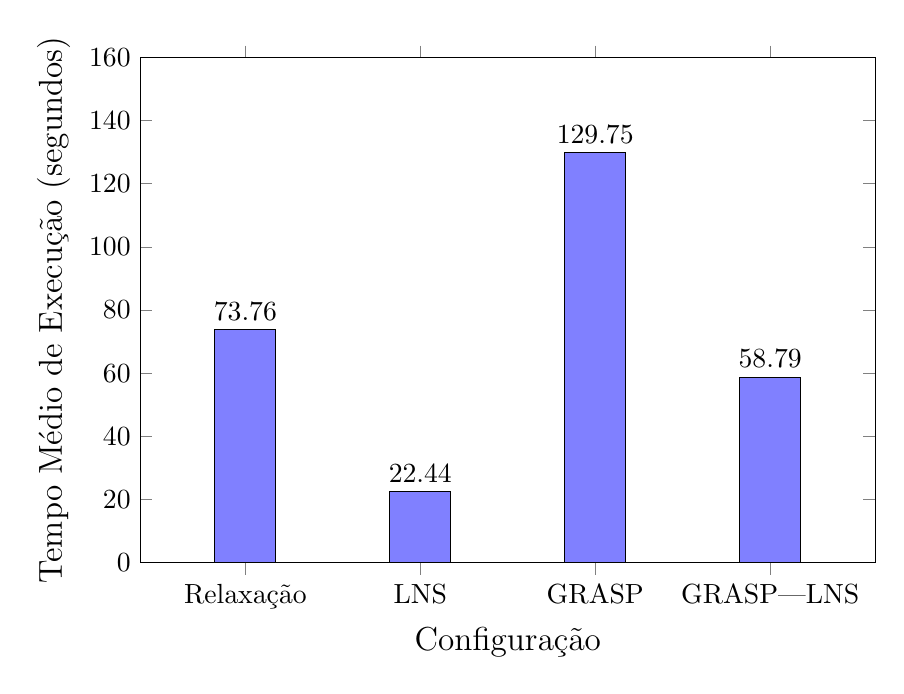
\begin{tikzpicture}
\begin{axis}[
    ybar,
    bar width=22pt,
    width=0.9\textwidth,
    height=8cm,
    ylabel={Tempo Médio de Execução (segundos)},
    xlabel={Configuração},
    symbolic x coords={Relaxação, LNS, GRASP, GRASP{|}LNS},
    xtick=data,
    nodes near coords,
    nodes near coords align={vertical},
    nodes near coords style={font=\normalsize, /pgf/number format/fixed,
        /pgf/number format/precision=2},
    ymin=0,
    ymax=160,
    enlarge x limits=0.2,
    ylabel style={font=\large},
    xlabel style={font=\large},
    tick label style={font=\normalsize},
]
\addplot[fill=blue!50] coordinates {
    (Relaxação,73.76)
    (LNS,22.44)
    (GRASP,129.75)
    (GRASP{|}LNS,58.79)
};
\end{axis}
\end{tikzpicture}
\caption{Tempo médio de execução (segundos) para cada configuração. O LNS obteve o menor tempo médio (22,44s), representando uma redução de 69,6\% em relação à relaxação pura e de 82,7\% em relação ao GRASP.}
\label{fig:geral_tempo}
\end{figure}
